\documentclass[border=4pt]{standalone}
\usepackage{tikz}
\usetikzlibrary{decorations.pathmorphing,arrows.meta}
\begin{document}
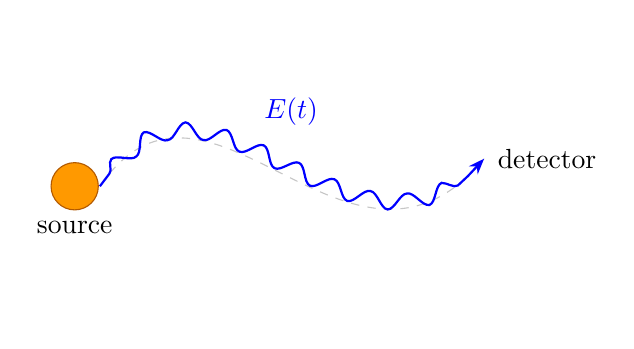
\begin{tikzpicture}
  \fill[orange!80!yellow] (-2.5,0) circle (3mm);
  \draw[orange!70!black] (-2.5,0) circle (3mm);
  \node[below] at (-2.5,-.32) {source};
  \draw[gray!45,dashed] (-2.18,0) .. controls (-.8,2.0) and (1.0,-1.7) .. (2.7,.35);
  \draw[blue,line width=.8pt,-{Stealth[length=2mm]},decorate,
    decoration={snake,pre length=2mm,post length=3mm,segment length=5mm,amplitude=1mm}]
    (-2.18,0) .. controls (-.8,2.0) and (1.0,-1.7) .. (2.7,.35);
  \node[blue,above] at (.25,.65) {$E(t)$};
  \node[right] at (2.75,.35) {detector};
\end{tikzpicture}
\end{document}
